\documentclass[First Project.tex]{subfiles}
\begin{document}

\subsection{ Τροποποιημένη μέθοδος της τέμνουσας }

Στην τροποποιημένη μέθοδο της τέμνουσας αλλάζει ο αναδρομικός τύπος της ακολουθίας για την εκτίμηση της ρίζας όπου χρησιμοποιούνται τρία
αρχικά σημεία αντί για δύο,  στην πραγματικότητα η μέθοδος βρίσκει μία παραβολή που περνάει και από τα τρία σημεία και ακολούθως βρίσκεται η 
τομή της παραβολής με τον άξονα $x$ όπου αποτελεί η νέα εκτίμηση της ρίζας, ενώ οι προϋποθέσεις της μεθόδου παραμένουν ίδιες(?). Η συνάρτηση 
\textit{\textlatin{\textbf{modified\_secant}}} από το αρχείο \textit{\textlatin{\textbf{modified\_secant.py}}} δέχεται τα ίδια ορίσματα με 
την κλασσική μέθοδο της τέμνουσας εκτός από την προσθήκη ενός ακόμα ορίσματος για το τρίτο αρχικό σημέιο \textlatin{\textbf{$x_{3}$}}. Ιδιαίτερη
προσοχή χρειάζεται στην επιλογή των αρχικών σημείων έτσι ώστε οι τιμές της \textlatin{\textbf{f(x)}} να είναι διακριτές και δύο από αυτές να 
έχουν αντίθετο πρόσημο καθώς αν για παράδειγμα στο πρώτο βήμα ισχύει \textbf{$f(x_{0}) = f(x_{2})$} δεν ορίζεται διαίρεση με το μηδέν και ο 
αλγόριθμος δεν μπορεί να συνεχίσει. Για την ρίζα της συνάρτησης στο διάστημα \textbf{[0.5,1.0]} επιλέγουμε τα αρχικά σημεία 
\textbf{$x_{0}$ = 0, $x_{1}$ = 0.5} και \textbf{$x_{2}$ = 0.75}.
\vspace{5px}
\begin{figure}[h!]
    \centering
    \captionsetup{justification=centering}
    \begin{center}
        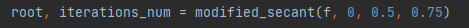
\includegraphics[scale=1]{exercise_2_secant_call_first_root.png}    
        \caption{ Παράδειγμα κλήσης της συνάρτησης \textit{\textlatin{\textbf{modified\_secant}}.}} 
    \end{center}
\end{figure}


Μετά την κλήση τα αποτελέσματα είναι τα εξής:
\vspace{5px}
\begin{figure}[h!]
    \centering
    \captionsetup{justification=centering}
    \begin{center}
    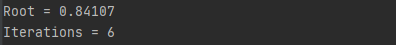
\includegraphics[scale=1]{exercise_2_secant_result_first_root.png}    
    \caption{ Αποτελέσματα κλήσης της συνάρτησης \textit{\textlatin{\textbf{modified\_secant}}} \\ με αρχικά σημεία \textbf{\textlatin{$x_{0}$ = 0}} 
                \textbf{\textlatin{$x_{1}$ = 0.5}} και \textbf{\textlatin{$x_{2}$ = 0.75}} . }
    \end{center}
\end{figure}

Ώπου παρατηρούμε ότι η ρίζα της \textlatin{\textbf{f(x)}} στο διάστημα \textlatin{\textbf{[0.5,1.0]}} με ακρίβεια 5 δεκαδικών ψηφίων 
είναι η \textbf{0.84107} καθώς και ότι η τροποποιήμενη μέθοδος της τέμνουσας χρειάστηκε \textbf{6} επαναλήψεις για να επιτύχει την 
επιθυμητή ακρίβεια. Για την ρίζα της \textlatin{\textbf{f(x)}} στο διάστημα \textlatin{\textbf{[2.0,2.5]}} επιλέγουμε τα αρχικά σημεία 
\textbf{$x_{0}$ = 1.5, $x_{1}$ = 1.8} και \textbf{$x_{2}$ = 2.3} κι έχουμε τα αποτελέσματα του \textit{Σχήματος 42}.
\vspace{5px}
\begin{figure}[h!]
    \centering
    \captionsetup{justification=centering}
    \begin{center}
    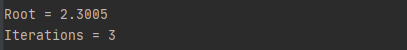
\includegraphics[scale=1]{exercise_2_secant_result_third_root.png}    
    \caption{ Αποτελέσματα κλήσης της συνάρτησης \textit{\textlatin{\textbf{modified\_secant}}} \\ με αρχικά σημεία \textbf{\textlatin{$x_{0}$ = 1.5}} 
                \textbf{\textlatin{$x_{1}$ = 1.8}} και \textbf{\textlatin{$x_{2}$ = 2.3}} . }
    \end{center}
\end{figure}

Ώπου παρατηρούμε ότι η ρίζα της \textlatin{\textbf{f(x)}} στο διάστημα \textlatin{\textbf{[2.0,2.5]}} με ακρίβεια 5 δεκαδικών ψηφίων 
είναι η \textbf{2.3005} καθώς και ότι η τροποποιήμενη μέθοδος της τέμνουσας χρειάστηκε \textbf{3} επαναλήψεις για να επιτύχει την 
επιθυμητή ακρίβεια. Τέλος, για την ρίζα της \textlatin{\textbf{f(x)}} στο διάστημα \textlatin{\textbf{[1.0,1.25]}} επιλέγουμε τα αρχικά σημεία 
\textbf{$x_{0}$ = 1.5, $x_{1}$ = 1.8} και \textbf{$x_{2}$ = 2.3} κι έχουμε τα παρακάτω αποτελέσματα :
\vspace{5px}
\begin{figure}[h!]
    \centering
    \captionsetup{justification=centering}
    \begin{center}
    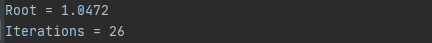
\includegraphics[scale=1]{exercise_2_secant_result_second_root.png}    
    \caption{ Αποτελέσματα κλήσης της συνάρτησης \textit{\textlatin{\textbf{modified\_secant}}} \\ με αρχικά σημεία \textbf{\textlatin{$x_{0}$ = 0.9}} 
                \textbf{\textlatin{$x_{1}$ = 1.1}} και \textbf{\textlatin{$x_{2}$ = 1.2}} . }
    \end{center}
\end{figure}

Ώπου παρατηρούμε ότι η ρίζα της \textlatin{\textbf{f(x)}} στο διάστημα \textlatin{\textbf{[1.0,1.25]}} με ακρίβεια 5 δεκαδικών ψηφίων 
είναι η \textbf{1.0472} καθώς και ότι η τροποποιήμενη  μέθοδος της τέμνουσας χρειάστηκε \textbf{26} επαναλήψεις για να επιτύχει την 
επιθυμητή ακρίβεια. Παρατηρούμε, ότι σε αυτή την περίπτωση ο αλγόριθμος χρειάστηκε αρκετές παραπάνω επαναλήψεις από τις άλλες ρίζες και αυτό
μάλλον οφείλεται στην πολλαπλότητα της συγκεκριμένης ρίζας και στην μορφή που έχει η συνάρτηση στην περιοχή γύρω από την ρίζα. 
\end{document}